\documentclass[journal]{IEEEtran}
\usepackage[a5paper, margin=10mm, onecolumn]{geometry}

\usepackage{gvv-book}
\usepackage{gvv}
\usepackage{cite}
\usepackage{amsmath,amssymb,amsfonts,amsthm}
\usepackage{algorithmic}
\usepackage{graphicx}
\usepackage{textcomp}
\usepackage{xcolor}
\usepackage{txfonts}
\usepackage{listings}
\usepackage{enumitem}
\usepackage{mathtools}
\usepackage{gensymb}
\usepackage{comment}
\usepackage[breaklinks=true]{hyperref}
\usepackage{tkz-euclide}
\usepackage{listings}
\usepackage{array}
\usepackage{longtable}
\usepackage{calc}
\usepackage{multirow}
\usepackage{hhline}
\usepackage{ifthen}
\usepackage{lscape}
\usepackage{tikz}
\usepackage{textcomp}
\usetikzlibrary{circuits.ee.IEC, positioning}

\begin{document}

\bibliographystyle{IEEEtran}
\vspace{3cm}

\title{11.16.1.4}
\author{Sai Akhila - EE24BTECH11055}

{\let\newpage\relax\maketitle}

\renewcommand{\thefigure}{\theenumi}
\renewcommand{\thetable}{\theenumi}
\setlength{\intextsep}{10pt}

\numberwithin{equation}{enumi}
\numberwithin{figure}{enumi}
\renewcommand{\thetable}{\theenumi}

\textbf{Question:} A fair coin is tossed and a fair six-sided die is rolled. Find the PMF of the random variable $X$, where $X$ is the sum of the number on the die and 1 if the coin lands heads, and the number on the die if the coin lands tails. Verify through simulation.\\

\textbf{Solution (Direct Calculation):}\\
Let $C$ be the outcome of the coin toss and $D$ be the outcome of the die roll. We have:

$C = \begin{cases} 1, & \text{if coin is heads} \\ 0, & \text{if coin is tails} \end{cases}$

$D \in \{1, 2, 3, 4, 5, 6\}$

$X = C + D$

The possible values for $X$ are $\{1, 2, 3, 4, 5, 6, 7\}$.

Since the coin and die are fair, we have:
$P(C=1) = 0.5$
$P(C=0) = 0.5$
$P(D=i) = \frac{1}{6}$ for $i \in \{1, 2, 3, 4, 5, 6\}$

Now we can calculate the PMF of $X$:
\begin{itemize}
    \item $P(X=1) = P(C=0, D=1) = P(C=0)P(D=1) = 0.5 \times \frac{1}{6} = \frac{1}{12}$
    \item $P(X=2) = P(C=0, D=2) + P(C=1, D=1) = (0.5 \times \frac{1}{6}) + (0.5 \times \frac{1}{6}) = \frac{2}{12} = \frac{1}{6}$
    \item $P(X=3) = P(C=0, D=3) + P(C=1, D=2) = (0.5 \times \frac{1}{6}) + (0.5 \times \frac{1}{6}) = \frac{2}{12} = \frac{1}{6}$
    \item $P(X=4) = P(C=0, D=4) + P(C=1, D=3) = (0.5 \times \frac{1}{6}) + (0.5 \times \frac{1}{6}) = \frac{2}{12} = \frac{1}{6}$
    \item $P(X=5) = P(C=0, D=5) + P(C=1, D=4) = (0.5 \times \frac{1}{6}) + (0.5 \times \frac{1}{6}) = \frac{2}{12} = \frac{1}{6}$
    \item $P(X=6) = P(C=0, D=6) + P(C=1, D=5) = (0.5 \times \frac{1}{6}) + (0.5 \times \frac{1}{6}) = \frac{2}{12} = \frac{1}{6}$
    \item $P(X=7) = P(C=1, D=6) = P(C=1)P(D=6) = 0.5 \times \frac{1}{6} = \frac{1}{12}$
\end{itemize}

\textbf{Solution (Using Z-transform):}

Let $C$ be the outcome of the coin toss (1 for Heads, 0 for Tails) and $D$ be the outcome of the die roll (1 to 6). Then $X = C + D$.

The Z-transform of $C$ is:
$$Z_C(z) = E[z^C] = 0.5z^0 + 0.5z^1 = 0.5 + 0.5z$$

The Z-transform of $D$ is:
$$Z_D(z) = E[z^D] = \frac{1}{6}(z^1 + z^2 + z^3 + z^4 + z^5 + z^6)$$

Since $C$ and $D$ are independent, the Z-transform of $X = C + D$ is:
$$Z_X(z) = Z_C(z)Z_D(z) = (0.5 + 0.5z)\frac{1}{6}(z + z^2 + z^3 + z^4 + z^5 + z^6)$$
$$Z_X(z) = \frac{1}{12}(1 + z)(z + z^2 + z^3 + z^4 + z^5 + z^6)$$
$$Z_X(z) = \frac{1}{12}(z + 2z^2 + 2z^3 + 2z^4 + 2z^5 + 2z^6 + z^7)$$

The coefficient of $z^k$ gives $P(X=k)$:
\begin{itemize}
    \item $P(X=1) = \frac{1}{12}$
    \item $P(X=2) = \frac{2}{12} = \frac{1}{6}$
    \item $P(X=3) = \frac{2}{12} = \frac{1}{6}$
    \item $P(X=4) = \frac{2}{12} = \frac{1}{6}$
    \item $P(X=5) = \frac{2}{12} = \frac{1}{6}$
    \item $P(X=6) = \frac{2}{12} = \frac{1}{6}$
    \item $P(X=7) = \frac{1}{12}$
\end{itemize}

Thus, the PMF is:

\begin{align}
P_X(x) =
\begin{cases}
    \frac{1}{12}, & x = 1 \\
    \frac{1}{6}, & x = 2 \\
    \frac{1}{6},  & x = 3 \\
    \frac{1}{6},  & x = 4 \\
    \frac{1}{6},  & x = 5 \\
    \frac{1}{6},  & x = 6 \\
    \frac{1}{12}, & x = 7 \\
    0, & \text{otherwise}
\end{cases}
\end{align}

\textbf{Simulation:}

We simulate this process as follows:
\begin{enumerate}
    \item Simulate the coin toss: Generate a uniform random number between $[0, 1)$. If the number is less than $0.5$, the coin is heads (C=1), otherwise tails (C=0).
    \item Simulate the die roll: Generate a discrete uniform random number between 1 and 6 (inclusive).
    \item Calculate $X = C + D$.
    \item Repeat steps 1-3 for a large number of trials (e.g., $10^5$ simulations).
    \item Count the occurrences of each possible value of $X$ (1 through 7).
    \item Divide the counts by the total number of trials to estimate the PMF.
\end{enumerate}

The graph below shows the comparison between the theoretically calculated and simulated PMF of the given random variable.

\begin{figure}[htbp]
    \centering
    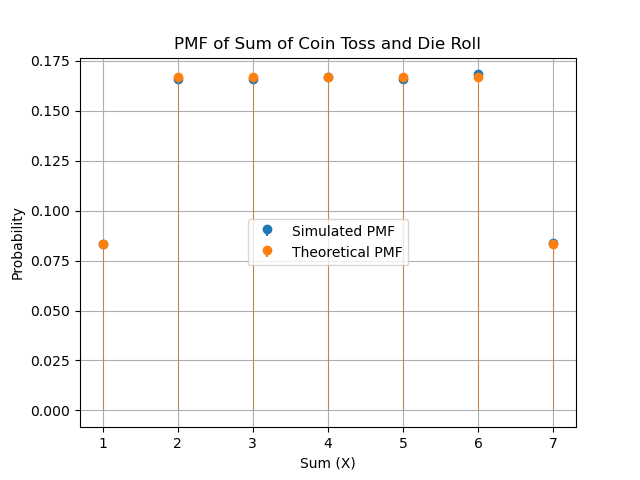
\includegraphics[width=\columnwidth]{fig/coin_die_pmf.png}
    \caption{Comparison of Theoretical and Simulated PMF}
\end{figure}

\end{document}

